
\begin{frame}[fragile]{Programming by Composition of Audio Circuits}

Faust is based on an algebra of 5 composition operations:
		
\begin{columns}
\column{0.5\textwidth}
\begin{center}
\lstinline'(A~B)'

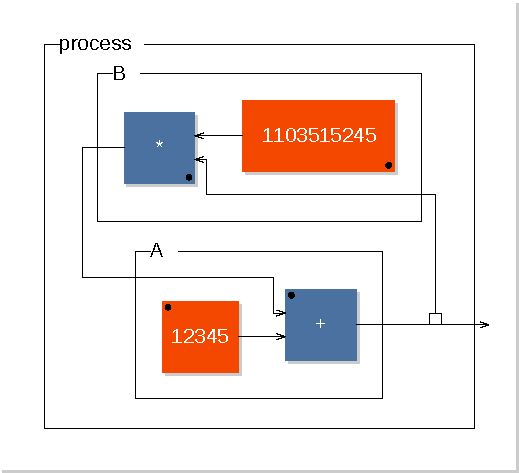
\includegraphics[height=3cm]{images/rec1} 
\end{center}

\column{0.5\textwidth}
\begin{center}
\lstinline'(A,B)'

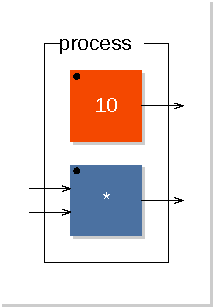
\includegraphics[height=3cm]{images/par1}
\end{center}

\end{columns}

\begin{columns}
\column{0.33\textwidth}
\begin{center}
\lstinline'(A:B)'

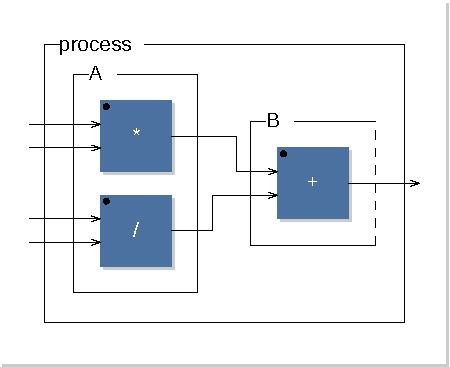
\includegraphics[height=3cm]{images/seq1} 
\end{center}

\column{0.33\textwidth}
\begin{center}
\lstinline'(A<:B)'

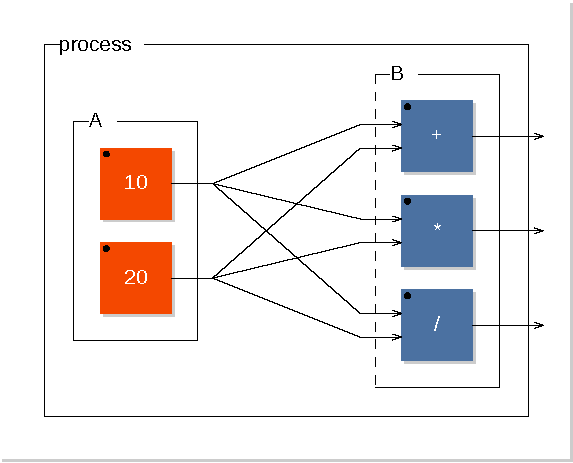
\includegraphics[height=3cm]{images/split1}
\end{center}

\column{0.33\textwidth}
\begin{center}
\lstinline'(A:>B)'

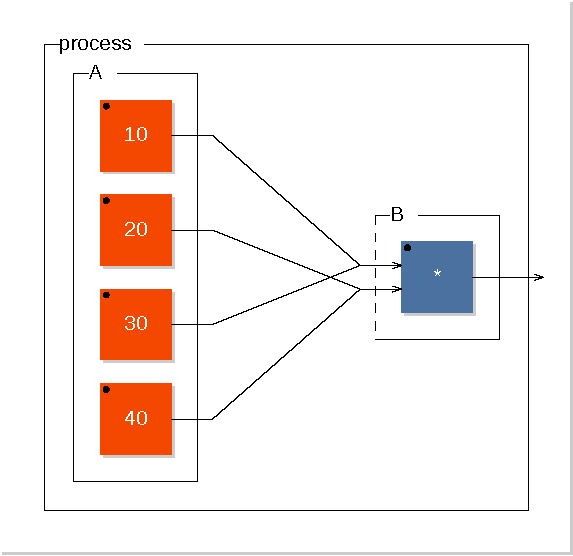
\includegraphics[height=3cm]{images/merge1}
\end{center}
\end{columns}



\end{frame}


